%%%%%%%%%%%%%%%%%%%%%%%%%%%%%%%%%%%%%%%%%
% Arsclassica Article
% LaTeX Template
% Version 1.1 (10/6/14)
%
% This template has been downloaded from:
% http://www.LaTeXTemplates.com
%
% Original author:
% Lorenzo Pantieri (http://www.lorenzopantieri.net) with extensive modifications by:
% Vel (vel@latextemplates.com)
%
% License:
% CC BY-NC-SA 3.0 (http://creativecommons.org/licenses/by-nc-sa/3.0/)
%
%%%%%%%%%%%%%%%%%%%%%%%%%%%%%%%%%%%%%%%%%

%----------------------------------------------------------------------------------------
%	PACKAGES AND OTHER DOCUMENT CONFIGURATIONS
%----------------------------------------------------------------------------------------

\documentclass[
10pt, % Main document font size
letterpaper, % Paper type, use 'letterpaper' for US Letter paper
%oneside, % One page layout (no page indentation)
twoside, % Two page layout (page indentation for binding and different headers)
headinclude,footinclude, % Extra spacing for the header and footer
]{scrartcl}

%%%%%%%%%%%%%%%%%%%%%%%%%%%%%%%%%%%%%%%%%
% Arsclassica Article
% Structure Specification File
%
% This file has been downloaded from:
% http://www.LaTeXTemplates.com
%
% Original author:
% Lorenzo Pantieri (http://www.lorenzopantieri.net) with extensive modifications by:
% Vel (vel@latextemplates.com)
%
% License:
% CC BY-NC-SA 3.0 (http://creativecommons.org/licenses/by-nc-sa/3.0/)
%
%%%%%%%%%%%%%%%%%%%%%%%%%%%%%%%%%%%%%%%%%

%----------------------------------------------------------------------------------------
%	REQUIRED PACKAGES
%----------------------------------------------------------------------------------------

\usepackage[
nochapters, % Turn off chapters since this is an article        
beramono, % Use the Bera Mono font for monospaced text (\texttt)
eulermath,% Use the Euler font for mathematics
pdfspacing, % Makes use of pdftex’ letter spacing capabilities via the microtype package
dottedtoc % Dotted lines leading to the page numbers in the table of contents
]{classicthesis} % The layout is based on the Classic Thesis style

\usepackage{arsclassica} % Modifies the Classic Thesis package

\usepackage[T1]{fontenc} % Use 8-bit encoding that has 256 glyphs

\usepackage[utf8]{inputenc} % Required for including letters with accents


\usepackage{filecontents}

%\usepackage{matlab-prettifier}

%\usepackage[framed,numbered,autolinebreaks]{mcode}

%\lstset{
%	style              = Matlab-editor,
%	basicstyle         = \mlttfamily,
%	escapechar         = ",
%	mlshowsectionrules = true,
%}

%\usepackage[colorlinks=true,citecolor=red,linkcolor=black]{hyperref}
\usepackage{hyperref}

\usepackage[citestyle=authoryear,bibstyle=authoryear,backend=biber,giveninits=true,maxcitenames=2,maxbibnames=99]{biblatex}

\usepackage{graphicx} % Required for including images
\graphicspath{{figures/}} % Set the default folder for images
\usepackage{wrapfig}

\usepackage{tikz}
\usepackage{pgfplots}
\pgfplotsset{compat=1.12}
\usepackage{tikz}
\usetikzlibrary{external}
\usetikzlibrary{decorations.shapes}
\tikzexternalize[optimize=false,prefix=cache/]
%\tikzset{external/force remake}
\newlength\figheight
\newlength\figwidth 

\usepackage{booktabs}
\usepackage{multirow}

\usepackage{nicefrac}
%\usepackage{units}
\usepackage[separate-uncertainty=true,multi-part-units=single]{siunitx}
%\usepackage{sistyle}

%\usepackage{enumitem} % Required for manipulating the whitespace between and within lists
\usepackage{enumerate}

\usepackage{lipsum} % Used for inserting dummy 'Lorem ipsum' text into the template

%\usepackage{subfigure} % Required for creating figures with multiple parts (subfigures)
\usepackage[justification=centering]{caption}
\usepackage{subcaption}

\usepackage{amsmath,amssymb,amsthm} % For including math equations, theorems, symbols, etc
\usepackage{varioref} % More descriptive referencing

\usepackage[left=1.5in,right=1in,top=1in,bottom=1in]{geometry}

\usepackage{url}

\usepackage{mathabx}

\usepackage{afterpage}

\usepackage{placeins}

%\usepackage{gensymb}

%\addbibresource{biblio_hmem.bib}
\addbibresource{bibliography.bib}


%----------------------------------------------------------------------------------------
%	THEOREM STYLES
%---------------------------------------------------------------------------------------

\theoremstyle{definition} % Define theorem styles here based on the definition style (used for definitions and examples)
\newtheorem{definition}{Definition}

\theoremstyle{plain} % Define theorem styles here based on the plain style (used for theorems, lemmas, propositions)
\newtheorem{theorem}{Theorem}

\theoremstyle{remark} % Define theorem styles here based on the remark style (used for remarks and notes)

%----------------------------------------------------------------------------------------
%	HYPERLINKS
%---------------------------------------------------------------------------------------

\hypersetup{
%draft, % Uncomment to remove all links (useful for printing in black and white)
colorlinks=true, breaklinks=true, bookmarks=true,bookmarksnumbered,
urlcolor=webbrown, linkcolor=RoyalBlue, citecolor=webgreen, % Link colors
pdftitle={heat_transfer_project}, % PDF title
pdfauthor={\textcopyright}, % PDF Author
pdfsubject={}, % PDF Subject
pdfkeywords={}, % PDF Keywords
pdfcreator={pdfLaTeX}, % PDF Creator
pdfproducer={LaTeX with hyperref and ClassicThesis} % PDF producer
}


%--------------------------------------------------------------------------------------
% OTHERS
%--------------------------------------------------------------------------------------

\newcommand*{\setiwonafont}{\fontfamily{iwona}\selectfont}

% Degree symbol
\newcommand{\degr}{\textsuperscript{\(\circ\)}} % Include the structure.tex file which specified the document structure and layout

\hyphenation{} % Specify custom hyphenation points in words with dashes where you would like hyphenation to occur, or alternatively, don't put any dashes in a word to stop hyphenation altogether

%--------------------------------------------------------------------------------------
%	TITLE AND AUTHOR(S)
%--------------------------------------------------------------------------------------

\title{\normalfont\spacedallcaps{Measurements of steady groundwater flow through granular material}} % The article title
 
\author{\spacedlowsmallcaps{Luc R\'ebillout, Yavuz \"Ozeren, Mustafa Altinakar}} % The article author(s) - author affiliations need to be specified in the AUTHOR AFFILIATIONS block

%\date{May, 9\textsuperscript{th} 2016} % An optional date to appear under the author(s)
%\date{\today}
\date{}

%----------------------------------------------------------------------------------------


\begin{document}

%--------------------------------------------------------------------------------------
%	HEADERS
%----------------------------------------------------------------------------------------

\renewcommand{\sectionmark}[1]{\markright{\spacedlowsmallcaps{#1}}} % The header for all pages (oneside) or for even pages (twoside)
\renewcommand{\subsectionmark}[1]{\markright{\thesubsection~#1}} % Uncomment when using the twoside option - this modifies the header on odd pages
\lehead{\mbox{\llap{\small\thepage\kern1em\color{halfgray} \vline}\color{halfgray}\hspace{0.5em}\rightmark\hfil}} % The header style

\pagestyle{scrheadings} % Enable the headers specified in this block

%----------------------------------------------------------------------------------------
%	TITLE, TABLE OF CONTENTS & LISTS OF FIGURES AND TABLES
%----------------------------------------------------------------------------------------

	\maketitle % Print the title/author/date block
	
%	{\centering\setiwonafont\itshape Draft ORSP	\\	
%		Report\\}
	
	\setcounter{tocdepth}{1} % Set the depth of the table of contents to show sections and subsections only
	
	\tableofcontents % Print the table of contents
	
%	\listoffigures % Print the list of figures
%	
%	\listoftables % Print the list of tables

%----------------------------------------------------------------------------------------
%	ABSTRACT
%----------------------------------------------------------------------------------------

\section*{Abstract} % This section will not appear in the table of contents due to the star (\section*)

This report presents the experimental findings of investigating flow inside a granular material in a rectangular channelized flume under constant head and at steady state. Manometers are distributed along the flume to measure the piezometric head of the flow while blue dye is added to make the water-air interface visible. Findings show that the water-air interface materialized by the blue dye is consistently higher than the piezometric surface and highlights the presence of a partially saturated capillary fringe above the piezometric surface.

%----------------------------------------------------------------------------------------
%	AUTHOR AFFILIATIONS
%----------------------------------------------------------------------------------------

%{\let\thefootnote\relax\footnotetext{* \textit{Department of Biology, University of Examples, London, United Kingdom}}}
%
%{\let\thefootnote\relax\footnotetext{\textsuperscript{1} \textit{Department of Chemistry, University of Examples, London, United Kingdom}}}

%----------------------------------------------------------------------------------------

\newpage % Start the article content on the second page, remove this if you have a longer abstract that goes onto the second page

%----------------------------------------------------------------------------------------
%	INTRODUCTION
%----------------------------------------------------------------------------------------

%\section{Introduction}
%


\section{Methodology}

Granular material is poured and leveled at a height of \SI{40}{cm} in a \SI{50}{cm} wide prismatic channel with transparent acrylic walls. In this experiment, granular particles of urea (plastic) are used to create the medium, Table \ref{tab:gran_mat} summarizes physical properties of this medium. The material is vertically contained upstream and downstream of the channel by a grid mounted with a fine mesh such as the water can freely penetrate the medium and exit by seeping out. Prior to the experiment, the channel is filled and drained a total of seven times to facilitate the packing and settling of the particles. The packing is likely not maximal and in situ cores of material [will be/are] retrieved along the channel to measure the bulk density of the medium and compare it with the bulk density of that same manually packed material measured in test tubes. 

The experiment begins by maintaining a constant head in the upstream reservoir so that water can infiltrate the medium. The system is then allowed to reach a steady state. Blue dye is mixed in the reservoir upstream to reveal the saturated portion of this laboratory unconfined aquifer. Manometers are evenly installed along the center line of the channel in order to monitor the piezometric head in the channel. Table \ref{tab:mano_pos} summarizes the hydraulic head measured by the manometers including the head in the reservoir. The water discharge is measured by collecting and weighing water downstream of the channel in a given amount of time; the unit mass discharge is $q = \dot{m} /W = \SI{0.728 \pm 0.039}{kg \cdot s^{-1} \cdot m^{-1}}$, $\dot{m}$ being the average mass discharge measured.

The profile created by the blue dye contrasting with the rest of the medium is manually selected using a \verb|livewire| tool implemented in Matlab by Christian Wuerslin based on an algorithm described in \cite{mortensen1995intelligent} that relies on graph cut segmentation.

\begin{table}[h]
	\caption{Material properties of Urea}
	\label{tab:gran_mat}
	\centering
	%						\resizebox{\linewidth}{!}{%
	\begin{tabular}{rc}
		\toprule
		$d_m$ [\SI{}{mm}]                                 & 2.05 \\
		$d_{90}$ [\SI{}{mm}]                              & 2.64 \\
		$d_{50}$ [\SI{}{mm}]                              & 2.24 \\
		$d_{10}$ [\SI{}{mm}]                              & 1.76 \\
		Internal angle of friction (direct shear test) $\phi$ [$^\circ$] & 38.4 \\
		Internal angle of friction (equilibrium slope) $\phi$ [$^\circ$] & 34.9 \\
		%			Internal angle of friction (dry dam break fitted slope) $\phi$ [$^\circ$] & 27 & 29 & 33.4 & 31.4 \\
		Bed friction angle $\delta$ [$^\circ$]            & 15.5 \\
		Specific Gravity [\textendash]                    & 1.51 \\
		Bulk density (packed) $\rho_b$ [\SI{}{kg/m^3}]    & 831  \\
		Hydraulic conductivity (packed) $K$ [\SI{}{mm/s}] & 8.51 \\
		Porosity  [\textendash]                           & 0.47 \\ \bottomrule
	\end{tabular}% 
	%						}
\end{table}

\begin{table}[h]
	\centering
	\caption{Location of manometers and piezometric head reading}
	\label{tab:mano_pos}
	\resizebox{\linewidth}{!}{%
		\begin{tabular}{rS[table-format=2.2]S[table-format=2.2]S[table-format=2.2]S[table-format=2.2]S[table-format=2.2]S[table-format=2.2]S[table-format=2.2]S[table-format=2.2]l}
			\toprule
			Id. & 1 & 2 & 3 & 4 & 5 & 6 & 7 & 8 & 9 $\left(\text{reservoir}\right)$ \\\midrule
			$x (m)$ & -0.12 & -0.42 & -0.72 & -1.02 & -1.32 & -1.62 & -1.92 & -2.22 & -2.57\\%\midrule
			Piezometric head $h (cm)$ & 7.5 & 14.1 & 18.7 & 22.7 & 25.8 & 28.8 & 31.3 & 34.0 & $35.3$ \\\bottomrule				
		\end{tabular}
	}
\end{table}

\section{Results \& Comments}

Figure \ref{fig:unconfined} shows an overview of the experiment along with the position of the manometers and the head measured ; a fit of the piezometric profile to the Dupuit equation with the hydraulic conductivity $K$ as parameter and a spline fit of that same profile. 

\subsection{Dupuit comparison}

The Dupuit equation for the discharge in a rectangular unconfined aquifer is:

\begin{align}
q = \frac{K}{2 \left(x_0 - x\right)}\left(h^2(x) - h_0^2\right)
\end{align}

Where $h_0$ and $x_0$ are a reference upstream head and location respectively and $h(x)$ is the head at location $x$. The upstream grid generating some head loss between the reservoir and the granular material, the reference head is chosen to be the one measured by manometer 8 (cf. Table \ref{tab:mano_pos}) for the purpose of curve fitting. In this case, the slope of the profile can approach 10\% which makes the Dupuit assumption non-valid for this case, however, it does provide an estimate for the in situ hydraulic conductivity i.e. $K = \SI{2.74}{cm/s}$ which is much greater than the one previously measured in packed material using a constant head method $K \text{ (packed)} = \SI{0.851}{cm \cdot s^{-1}}$.

\begin{figure}[h]
	\centering
	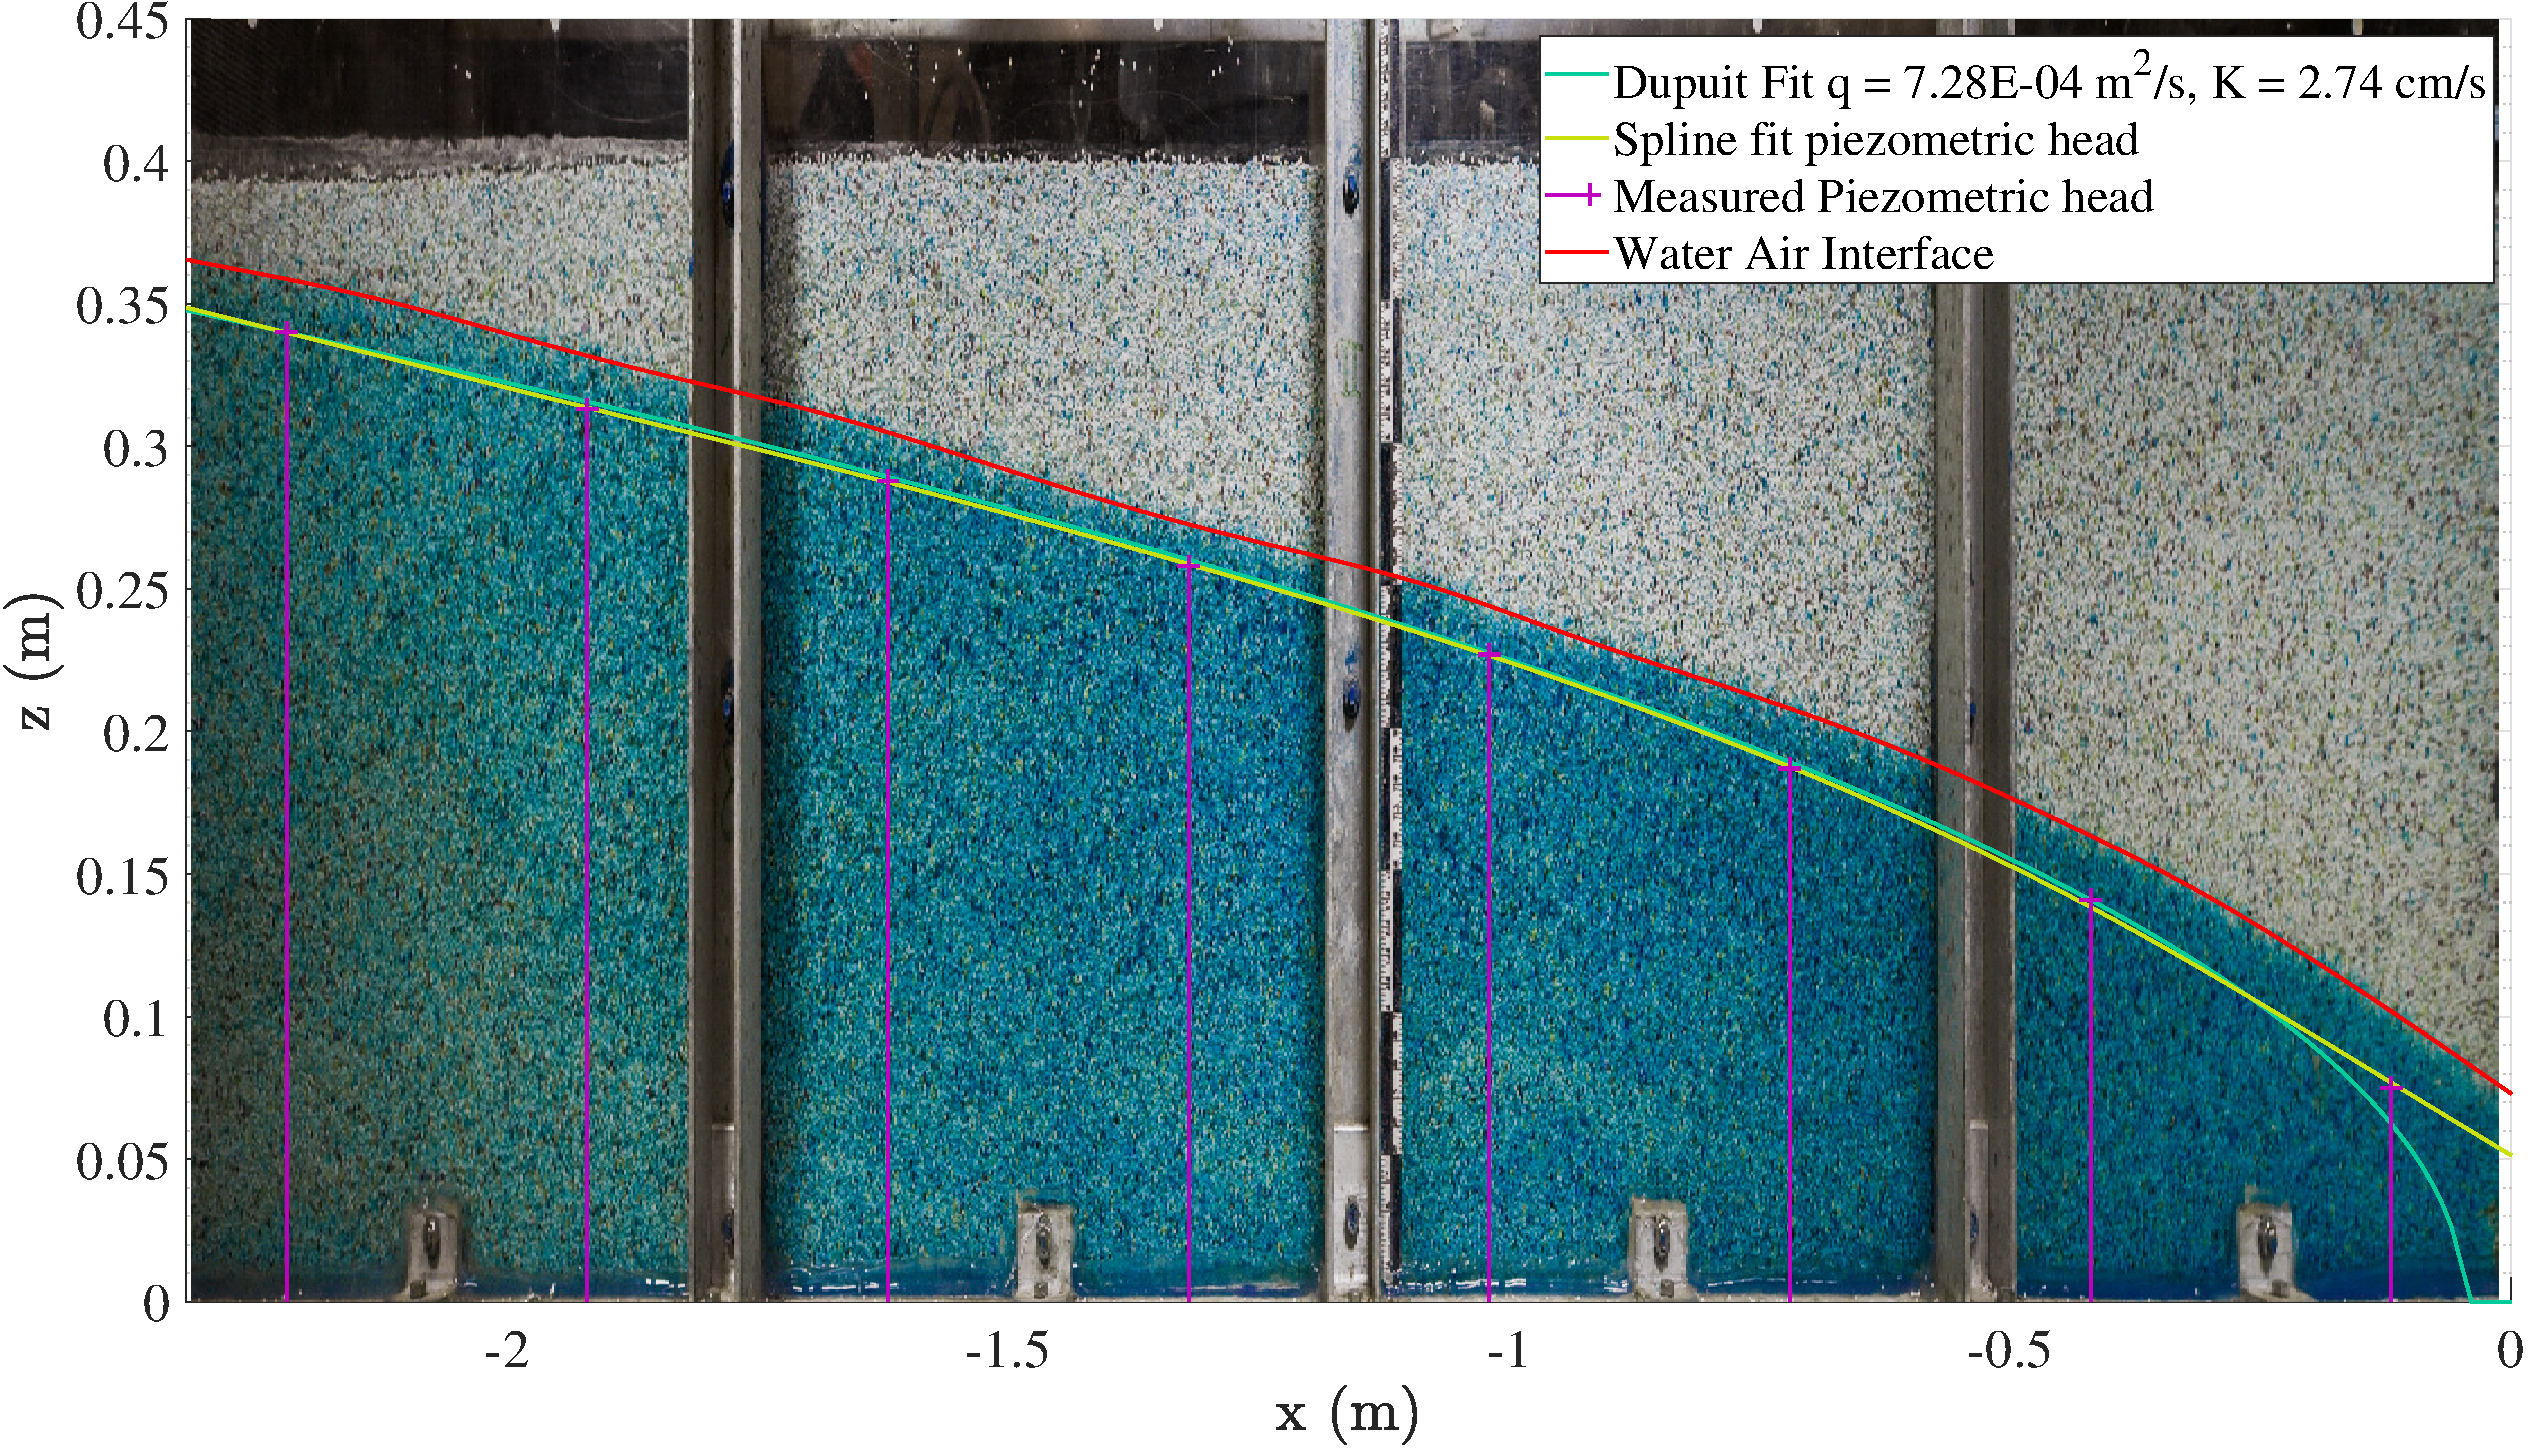
\includegraphics[width=0.95\linewidth]{figures/dupuit_mano_water_190209.pdf}
	\caption{Side view of the flume with piezometric surface and water-air interface}
	\label{fig:unconfined}
\end{figure}%

\subsection{Capillary fringe}

The height difference between the digitized profile materialized by the blue dye and the spline curve fitted through the piezometric head is reported in Figure \ref{fig:deltaH}. That height difference highlights the presence of a partially saturated capillary fringe above the piezometric surface. That difference varies along the flume between $1.39$ and \SI{2.68}{cm}. It is conjectured that the variation of the thickness of that capillary fringe is due to local variations in packing with some uncertainty also being due to the manual digitization of the profile.

\begin{figure}[h]
	\centering
	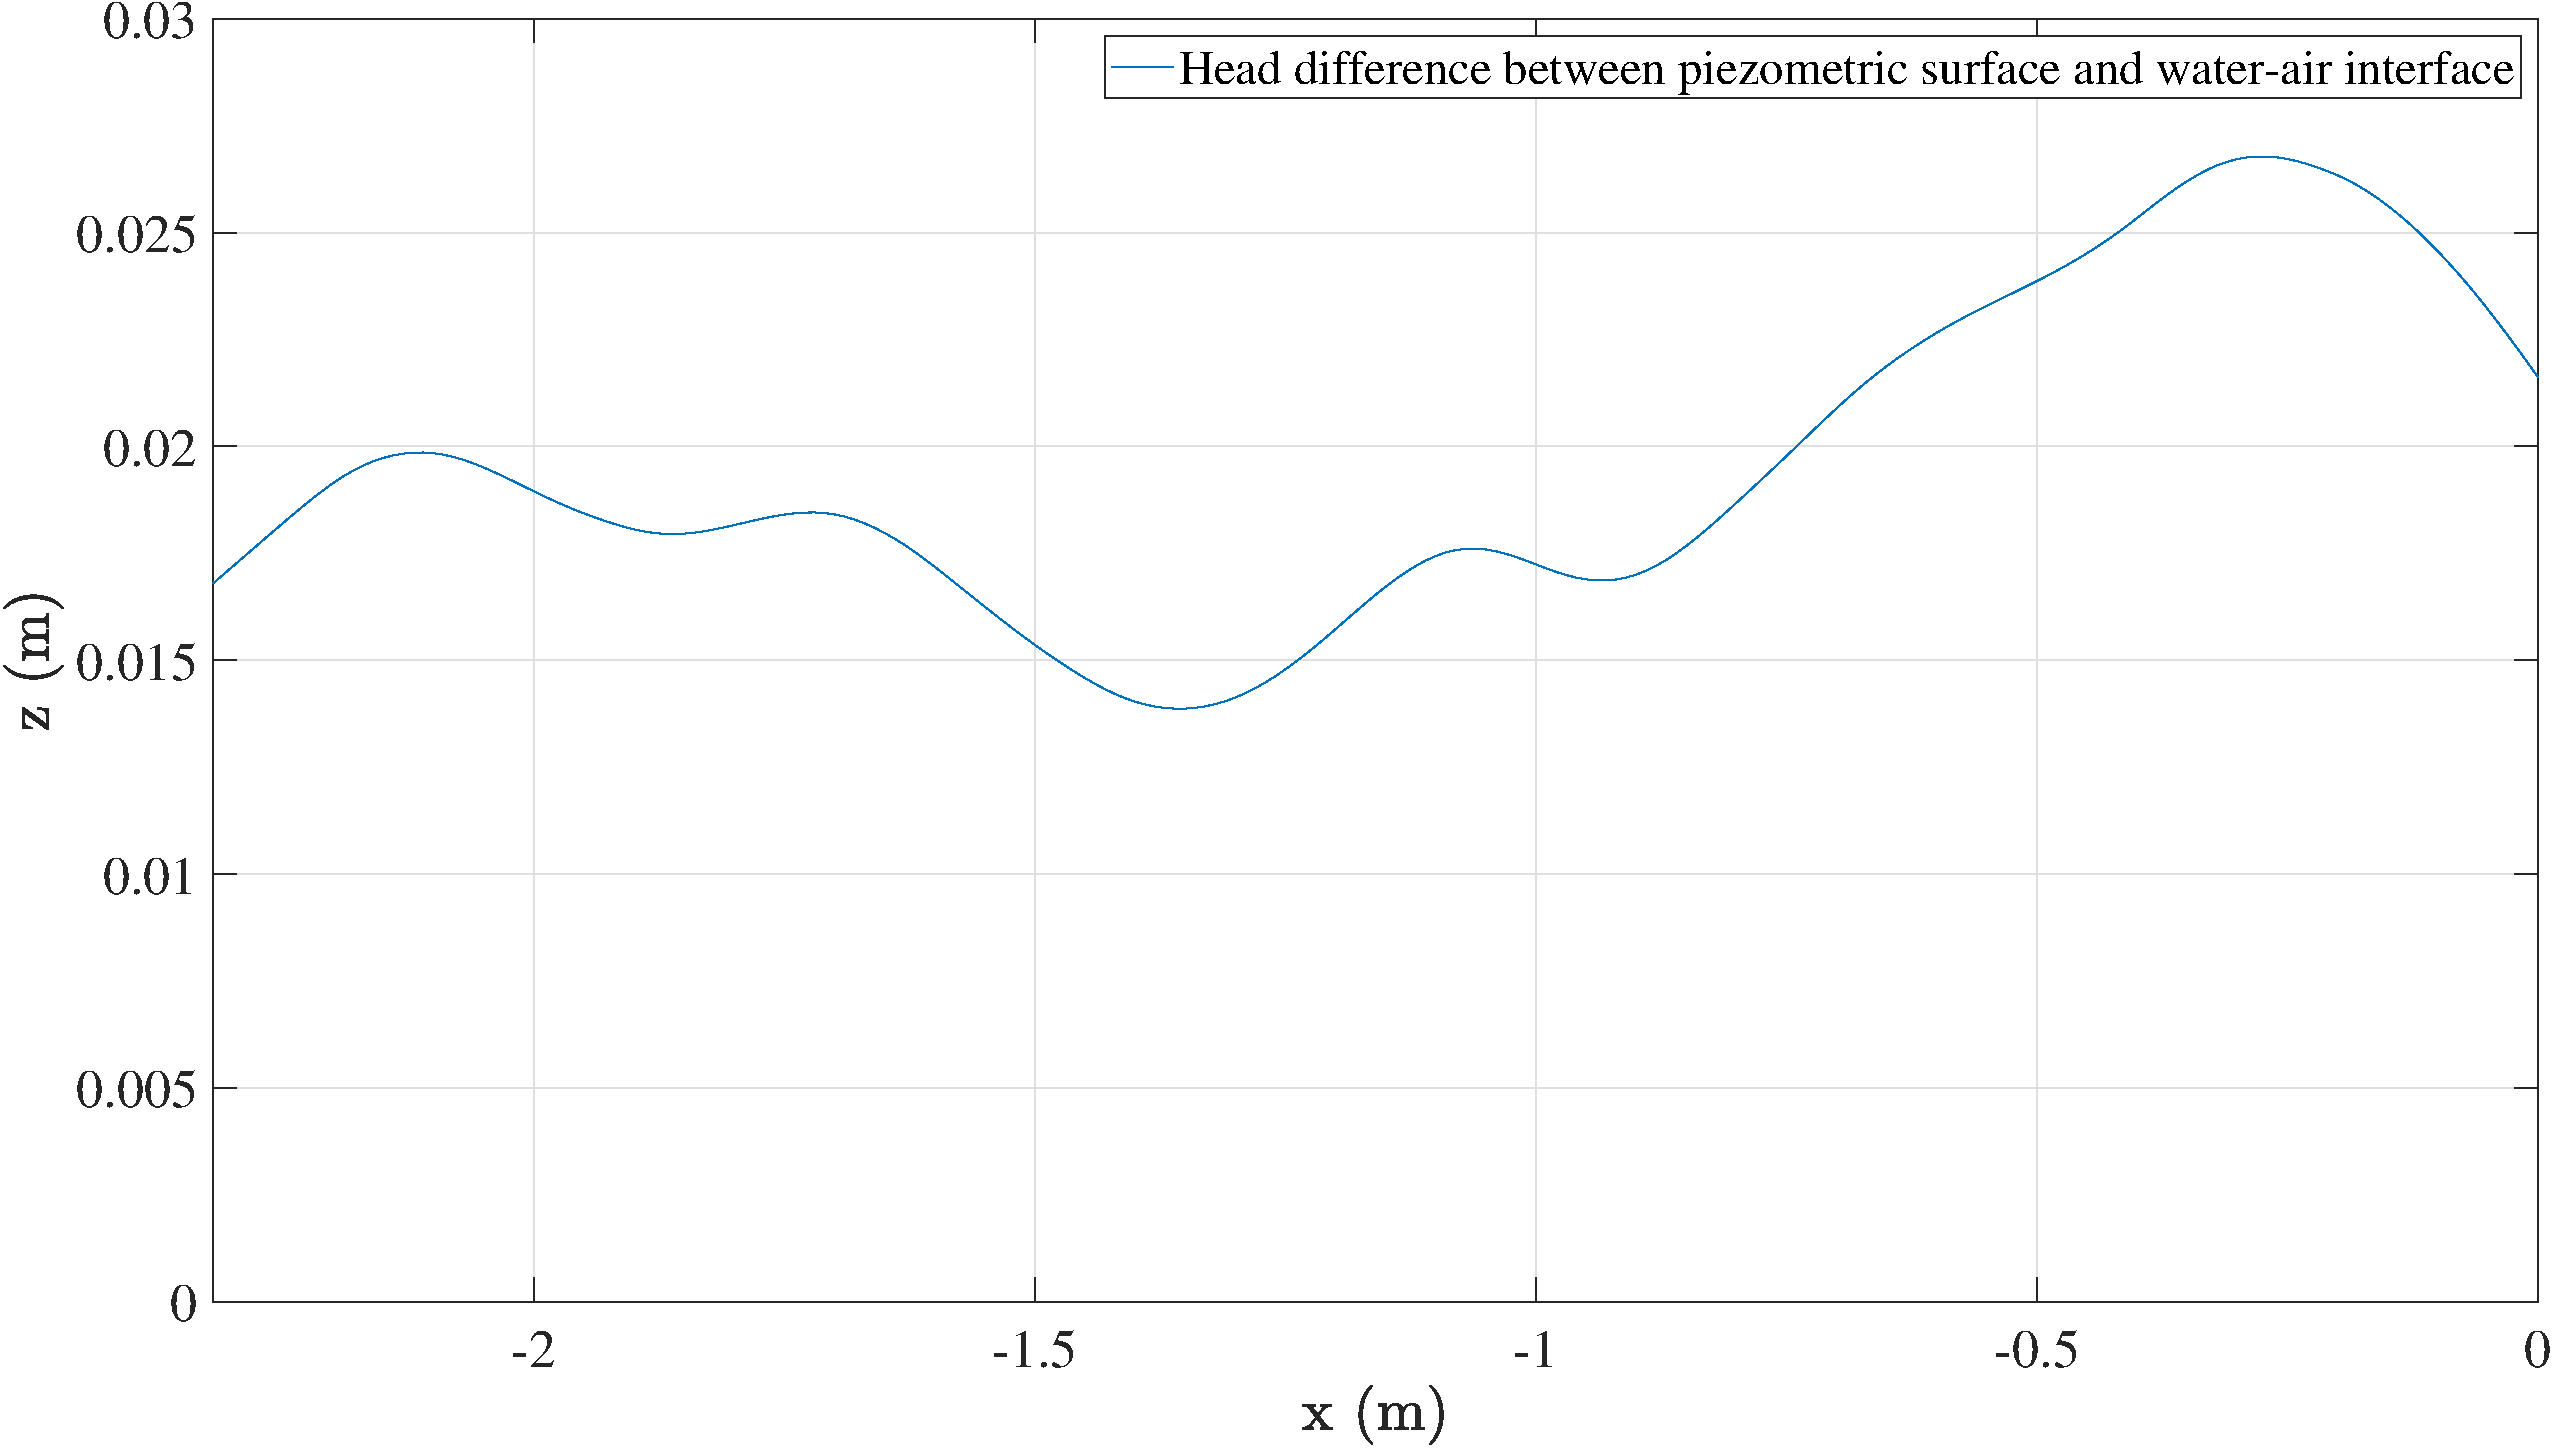
\includegraphics[width=0.75\linewidth]{figures/head_diff_190209.pdf}
	\caption{Height difference between the blue profile and the piezometric head profile}
	\label{fig:deltaH}
\end{figure}%

\FloatBarrier
\section{Conclusion}

This experiment allows to investigate the use of dye to track the evolution of flow inside an unconfined granular medium. It is shown that the dye does not highlight the phreatic surface but rather some area of the capillary fringe. Future investigation would require measuring the "Soil Moisture Characteristic Curve" of this synthetic material in order to know at which level of saturation the location of the dye corresponds to in order to have a better characterization of the unsaturated zone of the medium.

%\section{References}
%\nocite{*}
\clearpage
\printbibliography

\end{document}
